\documentclass[12pt]{article}
\usepackage[margin=.5in]{geometry}
\usepackage{setspace}
\usepackage{graphicx}

\begin{document}

\author{Dakota Szabo, Noah Zimmt}
\title{ Assignment \#5: \\
	\textbf{
		Throughput of Reduction Operations \\
		with MPI \& CUDA
	}
}
\maketitle



\begin{figure}
	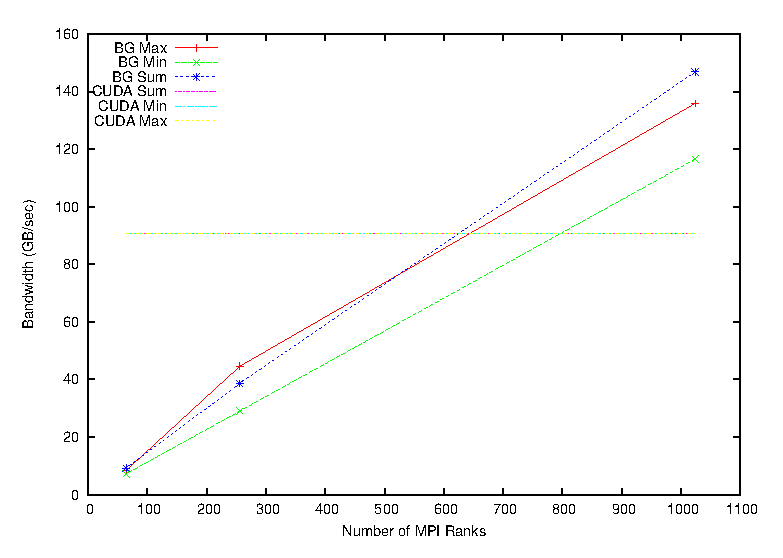
\includegraphics[width=\textwidth]{mpi/int.eps}
	\caption{Throughput of Integer Reductions}
\end{figure}

\begin{figure}
	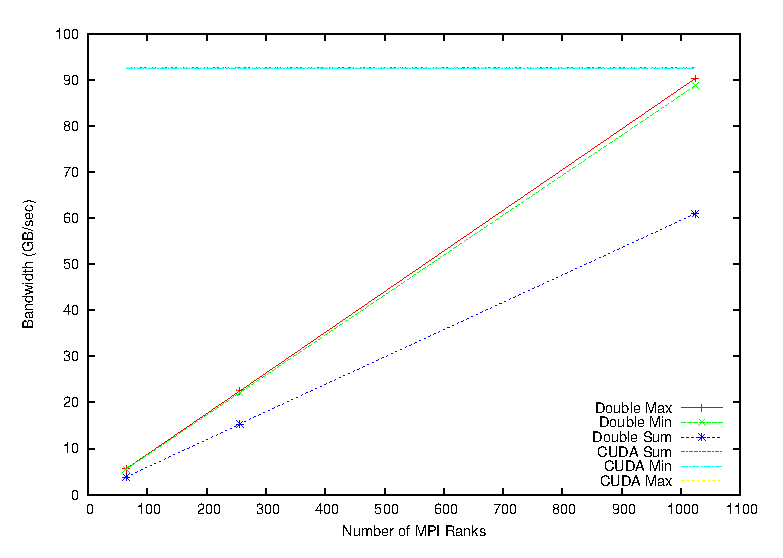
\includegraphics[width=\textwidth]{mpi/double.eps}
	\caption{Throughput of Double Reductions}
\end{figure}

Firstly, as can be seen from our data collected here, the CUDA reductions have a negligible difference in their overall bandwidth. This seems a little odd, but given that sum, min, and max are all relatively fast atomic operations, it is possible that they all run at a similar pace on the CUDA architecture. The brunt of the work during these reductions was dealing with the sheer amount of data, rather than the computational portion. Also surprising was the fact that double reductions were {\bf faster} than integer reductions on CUDA. After a little research, we found CUDA documentation stating that memory access was optimized for 256 byte memory reads, and that smaller reads would run slower. This is potentially the cause of doubles being slightly faster than ints. On BlueGene, double reductions were about half the speed of integer reductions - this logically makes sense, as doubles are twice the size of integers. Even though there was the same amount of data being utilized in both cases, operations on doubles are more expensive than similar operations on ints. Overall, CUDA was significantly better-performing on double reductions than BlueGene was, with bandwidth on 1024 cores approaching the CUDA bandwidth. However, for integers, BlueGene seems to begin to outperform CUDA around 500-600 MPI ranks.  
\end{document}
